\section{Strategies}
    \bigskip
	\subsection{Presentation du problème}
		\subsubsection{L'objectif}
			Dans cette partie, nous allons analyser les stratégies envisageables pour jouer à Pokemon. Notre objetif sera de créer une IA capable de jouer à pokemon de la 						manière la plus performante possible sans que le temps de calcul ne soit trop grand.

			Pour cela nous envisagerons d'abord des solutions simples qui s'appuient sur l'aléatoire et sur des règles simples, puis nous travaillerons sur des IA plus performantes 					qui reposent sur les algorithmes généraux présentés en cours et enfin nous essayerons d'améliorer ces algorithmes pour qu'ils s'adaptent mieux à notre jeu.
		\subsubsection{Difficultés liées au jeu pokemon}
			Dans le papier de recherchce \textbf{Learning complex games through self play - Pokémon battles} de \emph{Miquel Llobet Sanchez}, l'auteur cherche à créer une IA 					qui joue à pokemon via des algorithmes de parcours de graphe utilisant du deeplearning (solution qui est généralement celle utilisée pour le jeu pokemon).

			Ce jeu y est présenté comme un jeu qui représente un challenge pour les intelligences artificielles (même modernes) pour les raisons suivantes:
			\paragraph{L'atomicité des tours :}
				A chaque tour, les deux joueurs soumettent une action, et la résolution des actions se fait en même temps via un systeme de priorité des actions (voir règles 						du jeu). Il en résulte que le jeu ne peut pas réellement être représenté comme un arbre et que le plus souvent, les joueurs éxecutent leurs actions dans des états 							différents de celui dans lequel l'action à été choisie.
			\paragraph{Le coût de simulation :}
				Il faut 5 à 40 ms aux moteurs de simulation de bataille pokemons opens sources pour simuler un tour. Sachant que notre version sera vraisemblablement moins 							optimisée, le coût de simulation sera un facteur trés limitant dans le nombre d'états qui pourront être explorés par nos agents.
			\paragraph{Stochasticité :}
				Le jeu pokemon n'est pas un jeu déterministe, la chance influence fortement l'issue des tours. Elle intervient dans le système de priorité : deux pokemons qui 				ont la 	même vitesse auront une chance sur deux d'attaquer en premier si les attaques ont la même priorité (sachant que dans notre version, seule vive-attaque 
				a une priorité differente). Certaines attaques incorporent des facteurs chances comme Ebullition qui possède une chance sur trois de brûler l'adversaire, et les 							statuts aussi (exemple : un pokemon paralysé a une chance sur trois de ne pas attaquer). Un agent qui saura prendre en compte le facteur chance aura donc un 					avantage certain sur les autres agents.
			\paragraph{Le facteur de branchement :}
			 	Sans prendre en compte la Stochasticité, le facteur de branchement est de 4 à 9 (4 attaques et 5 changements potentiels).  Ce n'est pas comparable au facteur de 						branchement des échecs qui est en général autour de 35-38 mais cela reste non négligeable. D'autant plus que le facteur chance peut multiplier le nombre de 						branches par un coefficient compris entre 2 et 4 (ou plus dans de rares cas).
			\paragraph{Difficulté d'apréciation des etats}
					Certaines attaques comme piège de rock (pose des pièges qui inflige des dégâts à chaque changement de pokemon de l'adversaire) ont un effet sur le long 							terme qui sera difficile à apprecier pour les agents car ceux-ci seront forcement limités en terme de profondeur.
					De plus, les pokemons peuvent avoir un certain nombre de statut en même temps et de bonus qui vont être difficiles à apprécier.
    \subsection{Evaluation de l'état}
		Une fonction d'évaluation de l'état de bonne qualité est nécessaire pour créer des agents performants pour deux raisons principales. D'abord, c'est un outil trés intérressant 				pour évaluer les performances d'un agent. On pourra tracer le graphe de la fonction d'évaluation en fonction du nombre de tour lors d'un combat entre deux agents pour 					évaluer leurs performances tout au long de la partie. Ensuite, la fonction d'évaluation est necessaire à certains agents (ceux qui utilisent le minimax) pour avoir une 						approximation de l'utilité (les parties faisant en général plus de 30 tours, il est irréalisable de simuler la partie jusqu'à la fin pour ces agents).

		La fonction d'évaluation doit être rapide à calculer et representer le mieux possible l'état de la partie. Nous avons donc choisi de prendre la difference des PV de tout les 					pokemon du joueur 1 et de tout les pokemon du joueur 2.
		Le joueur max sera donc toujours le joueur 1 et le min le joueur 2 L'avantage c'est que cette fonction est rapide de calcul et 				représente bien ce qui est la clef de la victoire, les PV des pokemons.
		Le défault c'est quelle ne prend pas en compte les types des pokemon , leurs bonus et statuts, et leurs statistiques. Cependant tout ces éléments rajoutent du temps de 					calcul et demandent une connaissance du jeu que nous n'avons pas. Nous avons donc décidé de ne pas les prendre en compte.
		La prochaine étape pour améliorer nos agent serait d'entrainer un réseaux de neurone à évaluer chaque position. Qui sait c'est peut-être l'idée d'un futur projet, quand nous aurons les outils mathématiques nécessaires...
		\smallskip
		\paragraph{Implementation :}
		    (source : jeu.py): 
			\lstinputlisting[language=Python, tabsize=1,basicstyle=\scriptsize , linerange=valeur-end,includerangemarker=false]{code/jeu.py}
    \subsection{La classe joueur}
        Voici la classe joueur. Tout les agents sont des classes qui en héritent ce qui leur permet de connaitre quel dresseur de l'état ils representent (self.id) et de stocker les temps de réponse.
        
        \lstinputlisting[language=Python, tabsize=1,basicstyle=\scriptsize , linerange=Joueur-end,includerangemarker=false]{code/joueurs.py}
	\subsection{Solution envisagées}
		\subsubsection{Choix aléatoires}
			Une première solution serait de choisir aléatoirement une action parmi les mouvements autorisés. C'est une solution simple pratique pour tester le code avant 						d'envisager des solutions plus compliquées. Ce n'est bien sur pas une solution viable étant donné que pokemon est un jeu dans lequel seulement une petite partie 						des actions sont interressantes dans un etat donné. La probabilité de tomber aléatoirement sur une action viable est donc trop faible.
		\subsubsection{Règles simples}
			On donne à un agent des règles simples à suivre:
			\begin{itemize}
				\item Le premier pokemon est choisit au hasard
				\item Si le pokemon courant de l'agent n'a plus de pp sur ses attaques, il change de pokemon si possible.
				\item Si il y a un désavantage de type en faveur de l'adversaire, l'agent change de pokemon si possible.
				\item Quand il change de pokemon il essaye en premier de choisir un pokemon qui a un avantage de type par rapport à l'adversaire. Si il n'y en a pas, il choisit 						un pokemon qui n'a pas de désavantage de type. Si il n'y en a pas, elle essaye d'attaquer et si ce n'est pas possible elle change de pokemon au hasard. 
				\item Quand il attaque, l'agent fait toujours l'attaque qui fait le plus de dégat parmi les attaques qui ont des PP.
			\end{itemize}
			Ce sont des règles simples qui prennent comme priorité les PVs et les types des pokemons.
			\paragraph{Implementation :}
			    (source : joueurs.py): 
				\lstinputlisting[language=Python, tabsize=1,basicstyle=\scriptsize , linerange=avantage\_type-end,includerangemarker=false]{code/joueurs.py}
				\lstinputlisting[language=Python, tabsize=1,basicstyle=\scriptsize, linerange=basique-end,includerangemarker=false]{code/joueurs.py}
			\paragraph{Résultat :} 
				L'IA obtenue bat largement l'IA qui joue aléatoirement mais ne représente pas un grand défit pour un humain qui connait un peu le jeu.
				Elle bat largement l'IA aleatoire avec un temps de réponse de l'ordre de $10^{-9}$ avec de rares pics à $10^{-3}$ (tout les ordres grandeurs de temps sont 							pris avec le même ordinateur dans le même environnement de travail pour pouvoir les comparer).
				Exemple de partie jouées contre l'aléatoire :
		
				Sur 30 parties l'agent en gagne 30 et voici les valeurs des 2 premières parties:

				Première partie:

				Evolution de la valeur (l'agent qui utilise les règles est l'agent nommé basique en joueur 1 donc en max):
				Remarque : On peut voir le gagnant sur le graphique en regardant le signe du dernier point).

				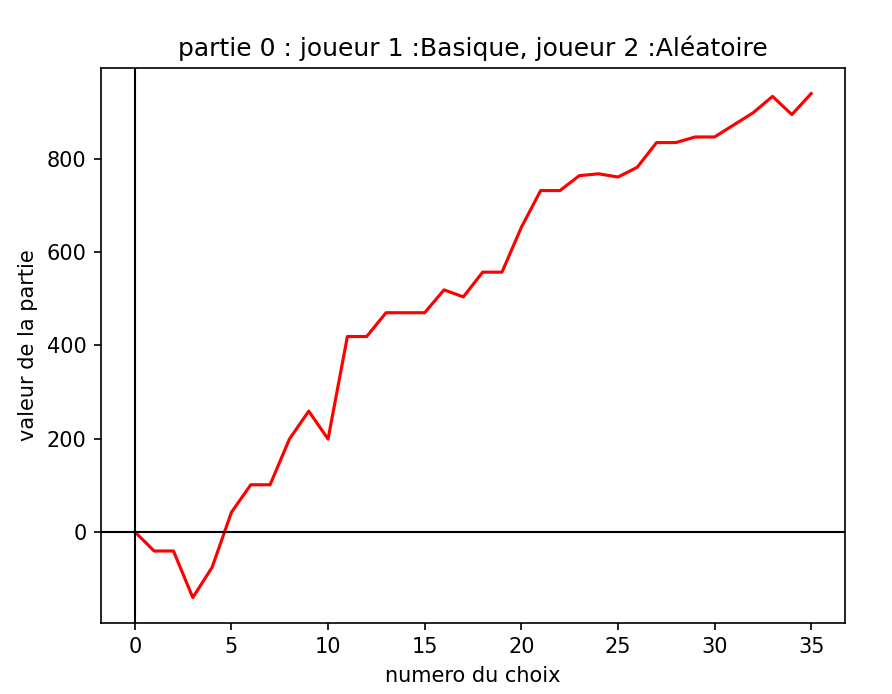
\includegraphics[width=4cm,height=4cm]{graphiques/valeur_basique_alea1}

				Seconde partie:

				Evolution de la valeur (l'agent qui utilise les règles est l'agent nommé basique en joueur 1 donc en max):

				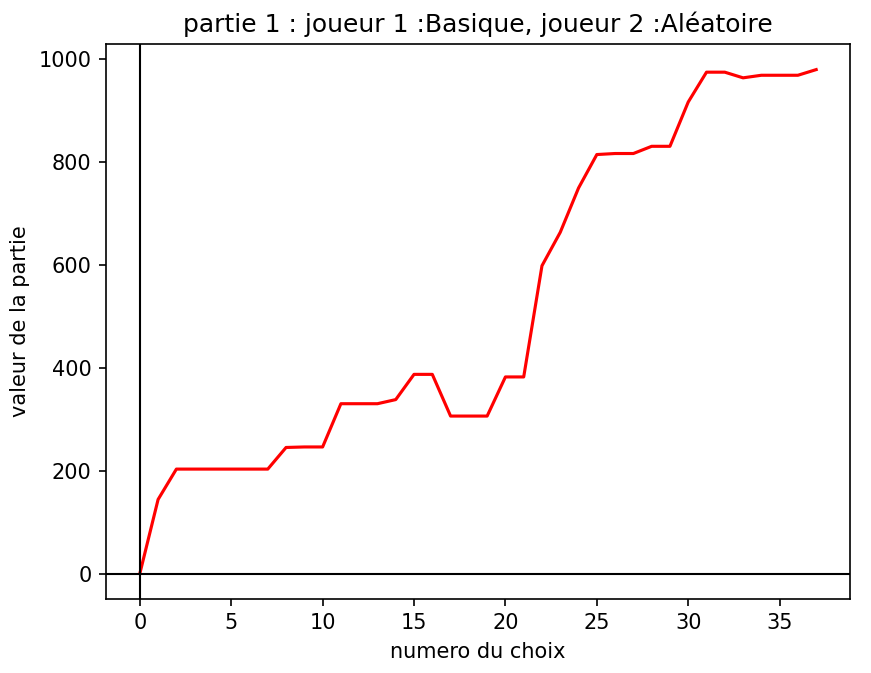
\includegraphics[width=4cm,height=4cm]{graphiques/valeur_basique_alea2}

				Le temps de réponse ne semble pas dépendre de la phase de la partie. Voici le temps de réponse au cours des 30 parties mises bout à bout:

				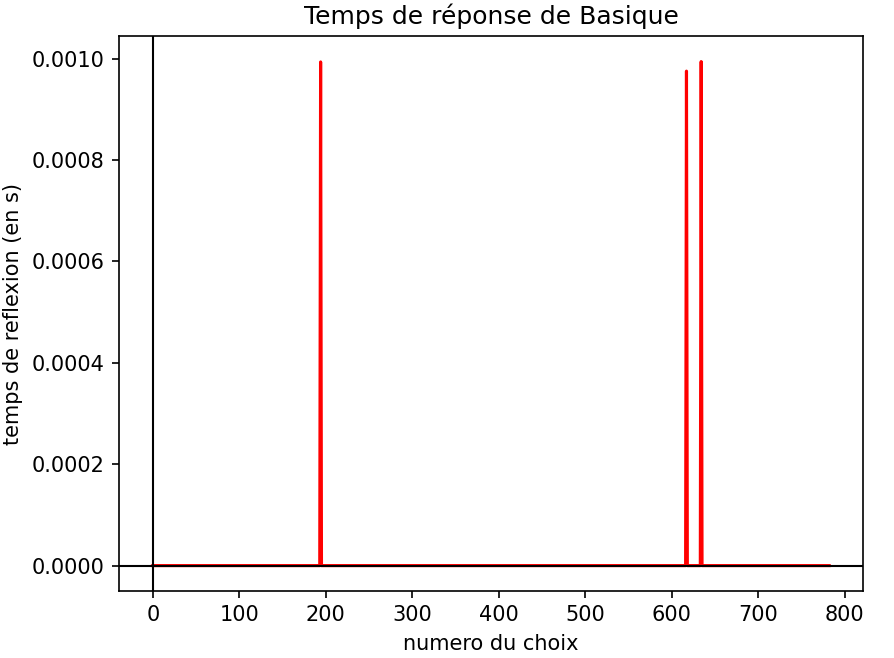
\includegraphics[width=4cm,height=4cm]{graphiques/temps_basique_alea1}

			\paragraph{Avantages :}
				Le temps de réponse et trés court. L'ia est trés forte contre des agents de bas niveau car elle cherche le plus possible à faire des dêgats.
			\paragraph{Défaults :}
				Le jeu pokemon et trop compliqué pour qu'un jeu de règles soit suffisant pour y être performant. Ces règles ne permettent pas de prendre en compte les 					spécificités de l'etat du jeu à un moment donné de la partie. Une règle qui est valable dans certaines situation peut être une grande erreur dans d'autres. Par 							exemple, changer de pokemon à chaque fois qu'il y a un désavantage de type n'est pas une bonne idée. Si le pokemon de l'adversaire a trés peu de PV et qu'on 					est plus rapide que lui, il vaut mieux attaquer pour le mettre KO car ainsi il ne pourra pas riposter (étant plus lent, l'adversaire attaque en second et ne pourra 						pas attaquer si il est mit KO). L'agent resultant a donc un comportement trés prévisible qui peut être anticipé par un adversaire humain et il a une trés 								mauvaise adaptation aux situations. 

				L'agent cherche en priorité à mettre des dêgats mais ne profite pas des avantages que représentent les bonus et les statuts. 

				Il faut avoir une bonne connaissance du jeu pour trouver des règles convenables. Donner des règles sur l'utilisation des statuts et des bonus est par exemple 							difficile commes ces éléments sont trés situationnels. Le choix du premier pokemon est aussi difficile.

				L'ia obtenue n'est pas généralisable et ne peut pas être réemployée dans des jeux similaires.
		\subsubsection{Minimax}
			L'algorithme du minimax est un algorithme pour les jeux à deux joueurs en tour par tour à choix alternés. Dans cet algorithme on considère que un joueur le max 						cherche à maximiser la valeur du jeu et un autre cherche à la minimiser.
			Dans cet algorithme, l'ordinateur visite l'arbre du jeu sur une certaine profondeur puis remonte les valeurs associées à chaques coup de la manière suivante :
			\begin{itemize}
				\item Si on est à la profondeur p ou si le jeu est fini, on renvoie une aproximation de la valeur du jeu (celle de la fonction d'évaluation).
				\item Si c'est au min de jouer, il choisit l'action qui minimise la valeur du jeu.
				\item Si c'est au max de jouer, il choisit l'action qui maximise la valeur du jeu.
			\end{itemize}

			Une amélioration de cet algorithme est l'algorithme alpha beta qui stocke en mémoire deux entiers, alpha et beta, qui stockent respectivement la plus grande valeur 						trouvée par le max et la plus petite trouvée par le min et permet d'élaguer l'arbre c'est à dire de ne pas visiter les branches qu'il est inutile de visiter (celle qui quoi 						qu'il arrive ne seront pas choisies par l'adversaire.)

			Notre objectif dans cette section va être de discuter d'une adaptation de l'algorithme alpha beta au jeu pokemon.
			
			\paragraph{Problème de l'ordre de jeu et de l'atomicité des tours:}
				L'ordre de jeu dans pokemon n'est pas alternatif car un choix peut être demandé aux deux joueurs ou à un seul (en cas de KO) sans ordre prédéfinit. Il faut 							donc passer par une fonction intermédiaire qui regarde qui doit jouer et :
				\begin{itemize}
					\item Si un seul joueur doit jouer, on applique l'algorithme du minimax habituel.
					\item Si deux joueurs doivent jouer, le choix de l'agent sera pour celui qui est \emph{le plus optimal quel que soit le choix de l'adversaire}.
				\end{itemize}
			    \smallskip    			Pour determiner quel est le choix \emph{le plus optimal quel que soit le choix de l'adversaire}, on parcourt les mouvements de disponibles pour l'agent et on applique 				l'algorithme du minimax habituel en considérant cette action comme choisie. Pour chaque mouvement l'adversaire va donc choisir l'action qui est la meilleure sachant 					que notre agent à choisit ce mouvement, il va choisir le meilleur contre à notre action. On va récupérer une valeur d'état associée à chaque mouvement et son 						meilleur contre (comme les 2 joueurs jouent, il faut deux actions pour déplacer l'etat) et en déduire la meilleure action.
    
    			Par exemple pour le max : On parcourt l'ensemble des actions disponibles pour le max. Pour chaque action, le min choisit l'action qui minimise la valeur de l'etat 						sachant l'action qui est jouée par le max. On recupére toutes les valeurs associées aux couples mouvements du max, meilleur contre du min et on choisit le couple qui                                                          
    			a la valeur la plus grande. Ainsi on a choisit l'action qui maximise la valeur de l'état même si le min choisit le meilleur contre de cette action.
    			
    			L'algorithme sera developpé de la même manière que le minimax habituel mais avec trois fonction qui s'entre-appellent au lieu de deux : il y aura la \emph{fonction interface}, la fonction \emph{min} et la fonction \emph{max}.
			\paragraph{Problème de la Stochasticité}
			    Comme nous l'avons vu dans la section 5.1.2, le jeu pokemon n'est pas un jeu déterministe. Cependant, dans un premier temps, nous considèreront que le facteur chance est négligeable. Cette agent traitera donc l'aléatoire de la manière suivante : lorsqu'un etat peut mener à plusieurs états différents via un facteur chance, un de ces états sera choisit en respectant les probabilités qui sont associées à chaque état. L'etat choisit sera considéré comme le seul etat possible, ce qui menera forcement à des erreurs dans l'évaluation de la valeur des futurs états.
            \paragraph{Implementation:}
                
                La classe \emph{JoueurMinimax} (tout les agents qui utilisent le minimax en héritent)(source : joueurs.py):
                
                \lstinputlisting[language=Python, tabsize=1,basicstyle=\scriptsize , linerange=JoueurMiniMax-end,includerangemarker=false]{code/joueurs.py}
                
                L'agent (source : joueurs.py):
                
                \lstinputlisting[language=Python, tabsize=1,basicstyle=\scriptsize , linerange=JoueurAlphaBeta1-end,includerangemarker=false]{code/joueurs.py}
                
                L'algorithme minimax (source : minimax.py): 
                \smallskip
				La fonction interface (on ne met que celle du joueur 1, celle du joueur 2 étant similaire mais inversée):
					    \lstinputlisting[language=Python, tabsize=1,basicstyle=\scriptsize , linerange=interface-end,includerangemarker=false]{code/minimax.py}
					    
				La fonction max (source : minimax.py): 
					    \lstinputlisting[language=Python, tabsize=1,basicstyle=\scriptsize , linerange=max-end,includerangemarker=false]{code/minimax.py}
				\smallskip
				La fonction de traitement de l'aleatoire (source : minimax.py): 
				\lstinputlisting[language=Python, tabsize=1,basicstyle=\scriptsize , linerange=alea-end,includerangemarker=false]{code/minimax.py}
			\paragraph{Résultats :}
			    Le coût des calculs et le facteur de branchement limite la recherche à 2 de profondeur ce qui reste interréssant étant donné que dans la plupart des coups, il faut regarder les mouvements possibles pour les deux joueurs (à cause de l'atomicité des tours).
			    
			    L'agent obtenu est plus performent que tout les agents précédents.
			    
			    Son temps de réponse est bien plus élevé que ceux des agent précedents(entre 3 en 20s).
			    Contrairement aux agents précédents, son temps de réponse depend de la phase de la partie. En fin de partie il y a moins de choix possibles donc moins de calculs à faire.
			    
			    Son comportement est trés cohérent ce qui est une bonne réussite car on ne lui a pas donné d'instruction préalable. Dans la plupart des cas il change de pokemon quand il y a un désavantage de type mais pas quand son adversaire est affaiblit et qu'il peut le finir parce qu'il est plus rapide. Quand il a un avantage il attaque. Il lui arrive d'utiliser des statuts comme la paralysie et vampigraine, et des bonus.
			    
			    Même si il bat l'IA basique, certaines partie contre cet agent sont trés sérrées car il lui arrive de faire des érreurs à cause du facteur chance.
			    
			    Le pokemon qu'il choisit en premier est pikachou. C'est un trés bon choix car il est rapide et il possède l'attaque change éclair qui lui permet de changer de pokemon tout en faisant des dêgats au cas où il serait en désavantage de type.
			    
			    Face à un humain, l'agent commence à être interressant : il bat les débutants et peut mettre en difficultée les joueurs intermédières (Exemple la première partie faite par un des concepteur contre cette ia n'a été gagné avec un seul pokemon restant).
			    
			    Voici un exemple de partie contre l'aléatoire:
			    
			    La valeur de la partie (l'agent est en position de max):
			    
			    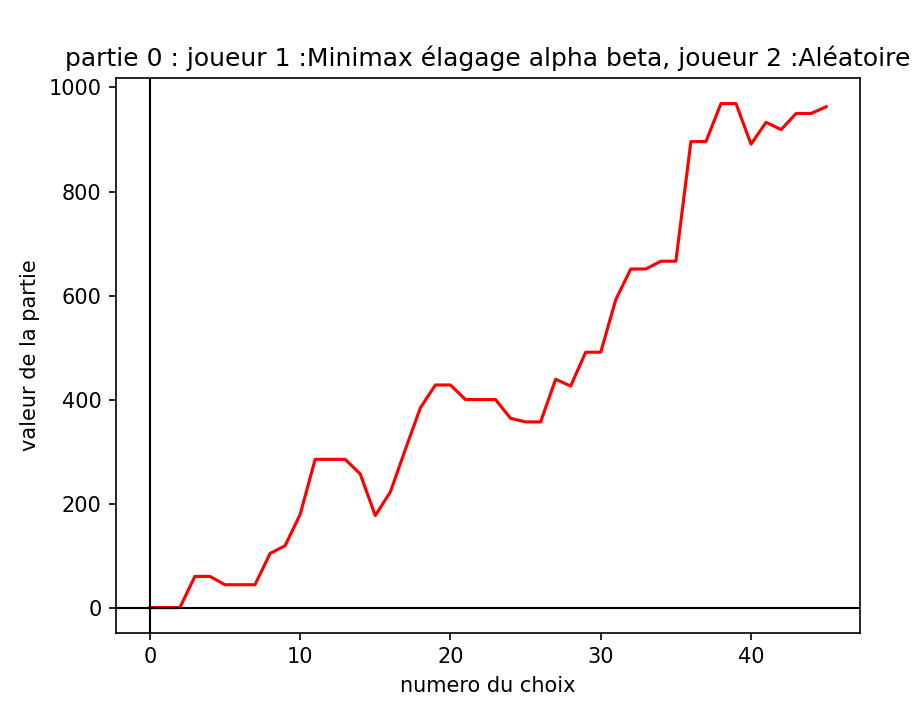
\includegraphics[width=4cm,height=4cm]{graphiques/valeur_alphbet_alea1}
			    
			    Le temps de réponse: On voit bien sur le graphique qu'il diminue en fin de partie.
                
                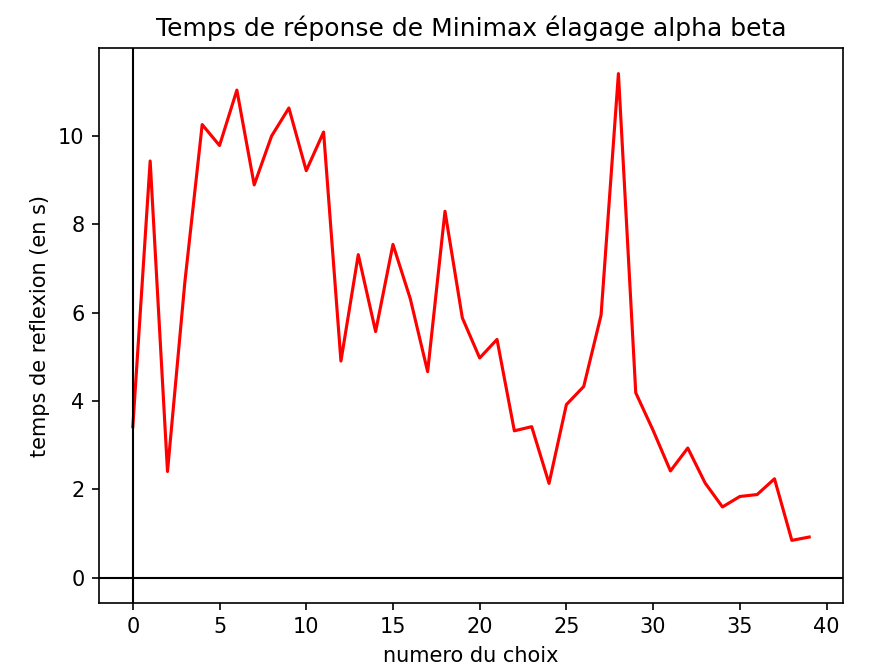
\includegraphics[width=4cm,height=4cm]{graphiques/temps_alphbet_alea1}
                
                Voici des exemples de partie contre l'ia basique (agent avec un jeu de règle):
			    
			    Deux exemples de la valeur de la partie (l'agent est en position de max):
			    
			    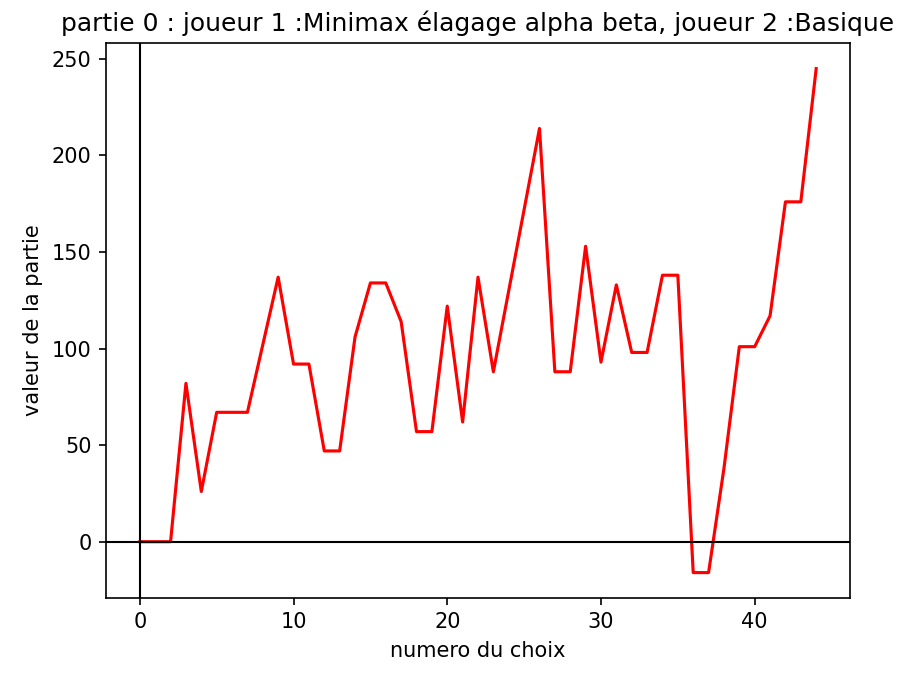
\includegraphics[width=4cm,height=4cm]{graphiques/valeur_alphbet_basique1}
			    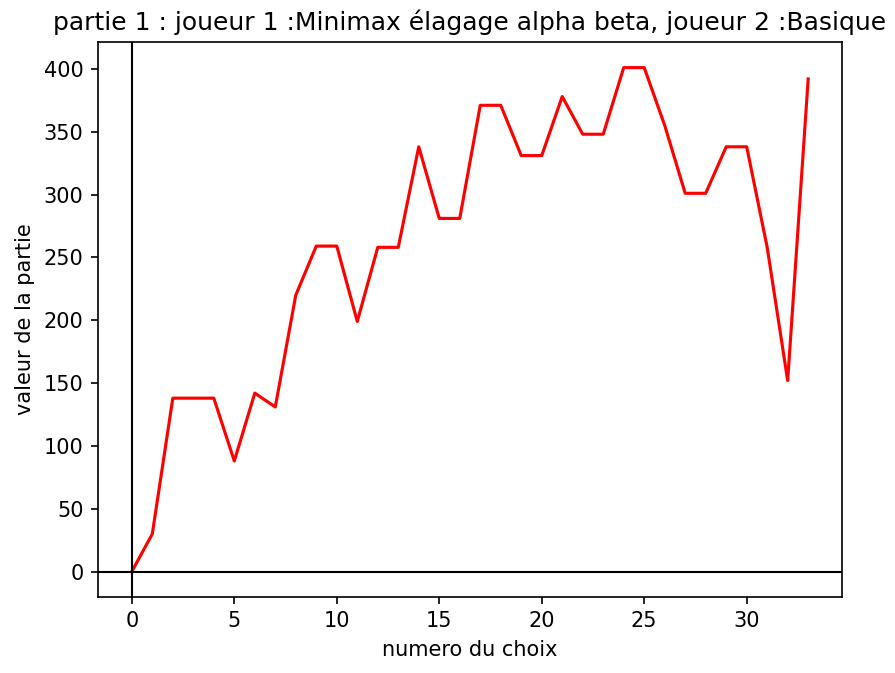
\includegraphics[width=4cm,height=4cm]{graphiques/valeur_alphbet_basique2}
			    
			    Un exemple de temps de réponse contre l'ia basique:
                
                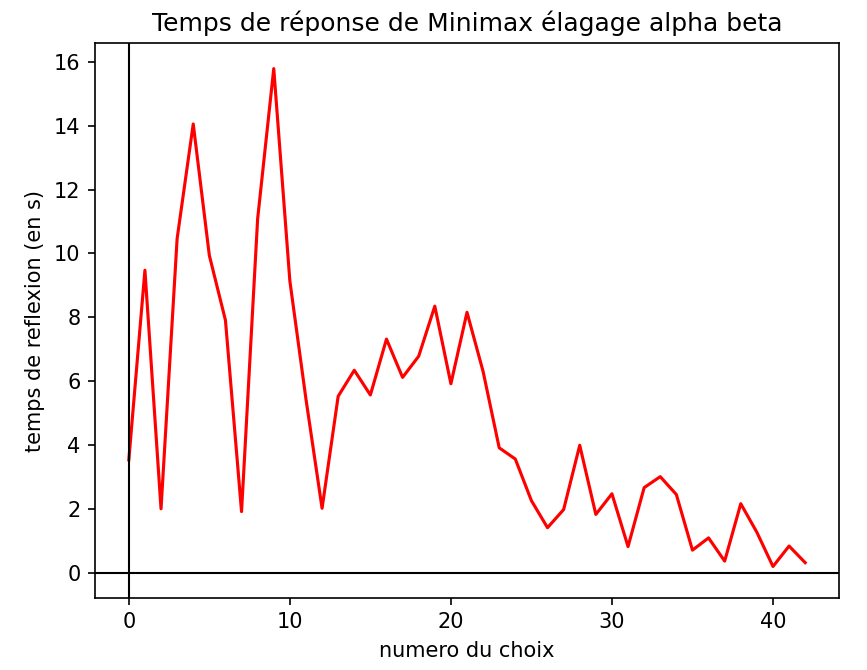
\includegraphics[width=4cm,height=4cm]{graphiques/temps_alphbet_basique1}
            \paragraph{Avantages :}
                L'agent n'est pas prévible comme il ne suit pas un jeu de règles.
                
                Il ne necessite pas de connaissance particulières dans le jeu et est généralisable à tout les jeux similaires à pokemon (jeu avec atomicité des tours et Stochasticité).
                
                Il est plus performant que tout les agents précédents et surtout en fin de partie.
                
                L'agent n'utilise pas que des attaques qui font des dêgats à court terme, il utilise aussi des statuts et des bonus.
            \paragraph{Desavantages :}
                Le temps de réponse de l'agent est assez important. Si on voulait créer une application dans laquelle des joueurs jouent contre notre ia, il serait difficile de leur faire accepter ce delai.
                
                L'agent à du mal à traiter l'aléatoire ce qui l'amène à faire des erreurs.
                
                La faible profondeur de recherche limite la comprehension réelle de l'état du jeu et empêche l'utilisation d'attaques à trés long terme comme piège de rock
                
                L'agent est trés prévisible en début de partie, sachant qu'il prend toujours pikachou en premier, l'adversaire peut choisir son contre.
                
        \subsubsection{Expectiminimax}
            Dans cette section on va apporter une amélioration à l'algorithme alpha beta afin de mieux traiter le facteur chance : l'expextiminimax.
            Pour ce faire, nous allons simplement changer la fonction de traitement de la chance : à chaque foix qu'il y aura plusieurs états possibles pour une action, la valeur de cette action sera l'esperance des valeurs de tout les états.
            \paragraph{Implementation:}
                
                Seule la fonction de traitement de l'aléatoire change:
                
                L'agent (source : joueurs.py):
                
                \lstinputlisting[language=Python, tabsize=1,basicstyle=\scriptsize , linerange=JoueurAlphaBeta2-end,includerangemarker=false]{code/joueurs.py}
                
                La fonction de traitement de l'aleatoire (minimax.py):
                
                \lstinputlisting[language=Python, tabsize=1,basicstyle=\scriptsize , linerange=esperance-end,includerangemarker=false]{code/joueurs.py}
                
            \paragraph{Résultats :}
                Le temps de reponse est plus élevé car il faut traiter en plus les branches liées à la chance. Il faut en général entre 10 et 30 secondes pour repondre. Cependant contrairement à l'agent précédent, il arrive que le temps de réponse l'ia expectiminimax stagne voire augmente en fin de partie. L'explication c'est qu'en fin de partie il y a plus de branches liées à la chance. L'augmentation du nombre de branches liées à la chance s'explique par l'augmentation du nombre de situation ou les deux pokemon sur le terrain ont des statuts. En effet, dans ce cas là, si les deux pokemons ont la même vitesse, la chance est à utilisée une première fois pour determiner qui attaque en premier et une seconde fois pour determiner qui subit les statuts en premier. Il y a donc plus de quatres etats possibles.
                
                Ensuites, les performances de l'agent sont superieures. En effet, grâce à sa maitrise du facteur chance cet agent bat tout les agents précédents.
                
                Les agents alea et basique sont battuts avec un écart de PV trés élevé mais en plus de tour qu'il n'en failait à l'agent minimax pour les battre. Cela montre que l'agent expectiminimax prend moins de risque mais au final est plus précis.
                
                Comme pour l'agent précédent, l'agent expectiminimax choisit pikachou en premier ce qui semble confirmer que c'est un bon choix.
                
                Son comportement et plus cohérent que tout les agents précédents car il ne fait pas d'erreurs liées au facteur chance.
                
                Face à un humain, l'agent est interressant : il bat les débutant et peut mettre en difficultée voire battre les joueurs intermédières.
                
                Voici un exemple de partie contre l'ia basique (agent avec un jeu de règle):
			    
			    La valeur de la partie (l'agent est en position de max) est à droite et le temps de réponse à gauche (On est dans le cas ou il ne diminue pas en fin de partie):
			    
			    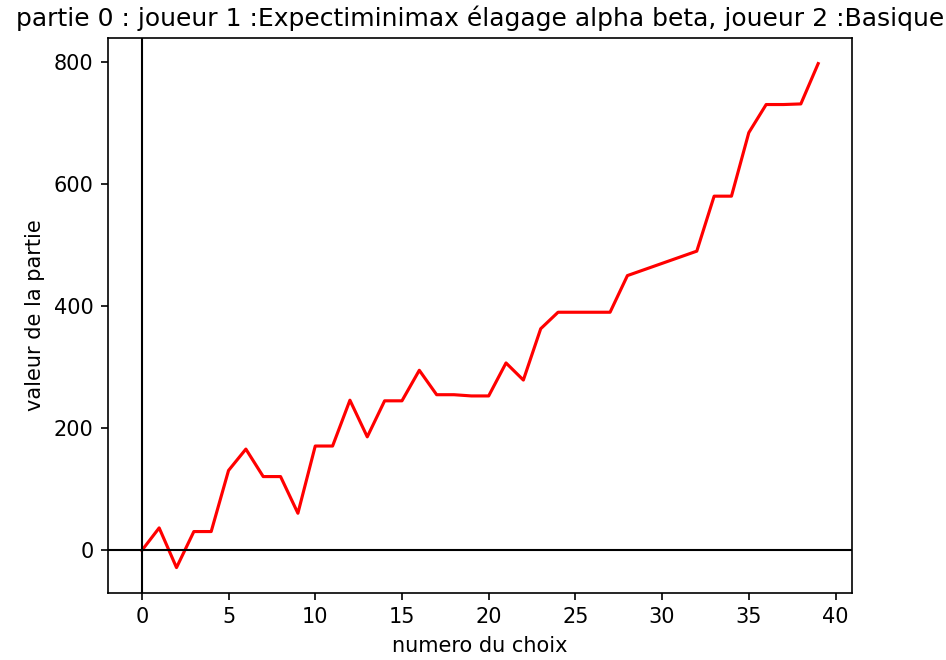
\includegraphics[width=4cm,height=4cm]{graphiques/valeur_alphbet2_basique1}                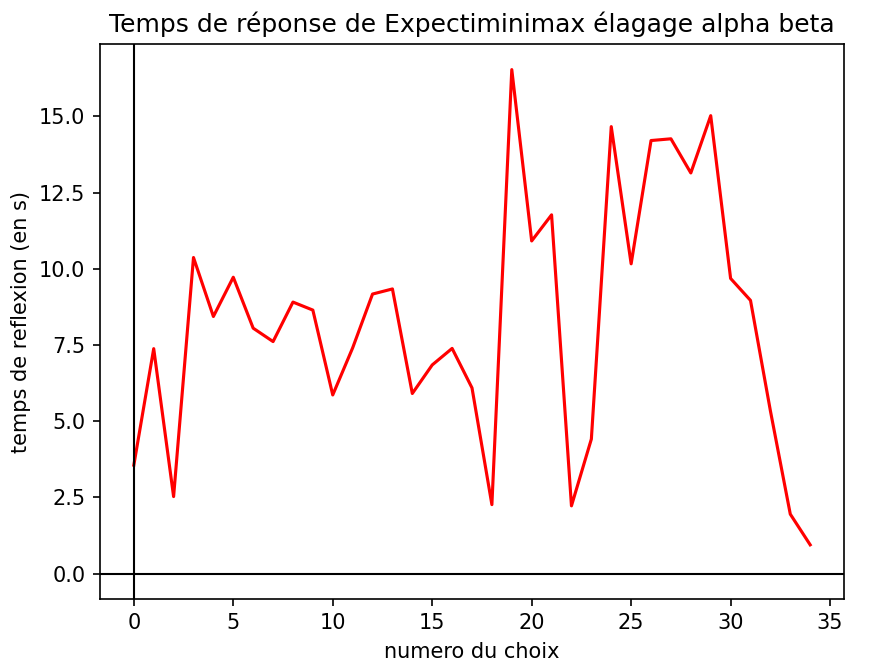
\includegraphics[width=4cm,height=4cm]{graphiques/temps_alphbet2_basique1}
                
                Voici deux exemples de partie contre l'ia alpha beta classique:
			    
			    Les valeur de la partie (l'agent expectiminimax est en position de max):
			    
			    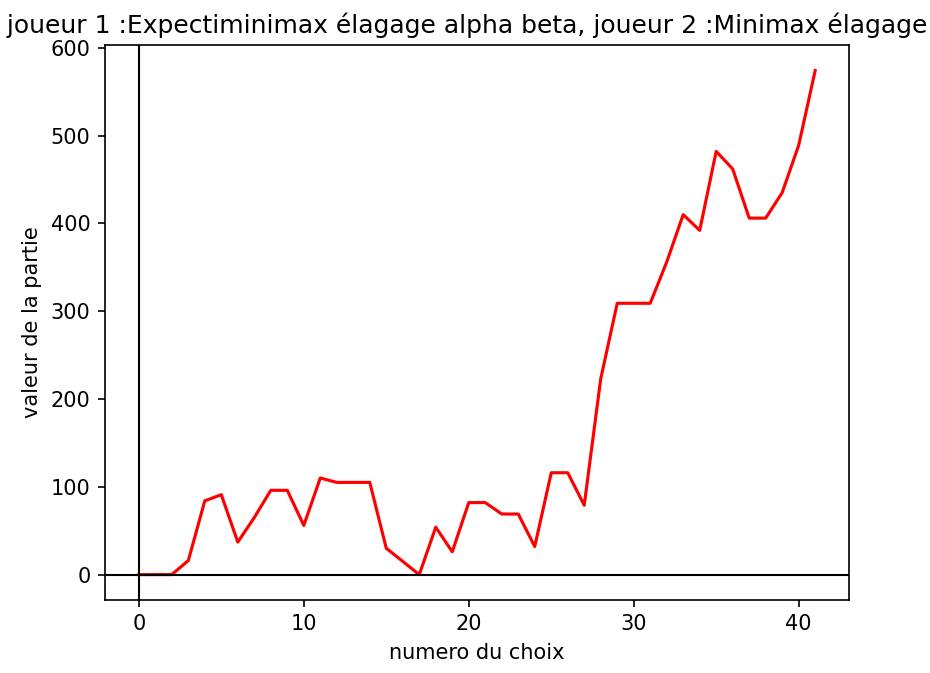
\includegraphics[width=4cm,height=4cm]{graphiques/valeur_alphbet2_alphabet1}
			    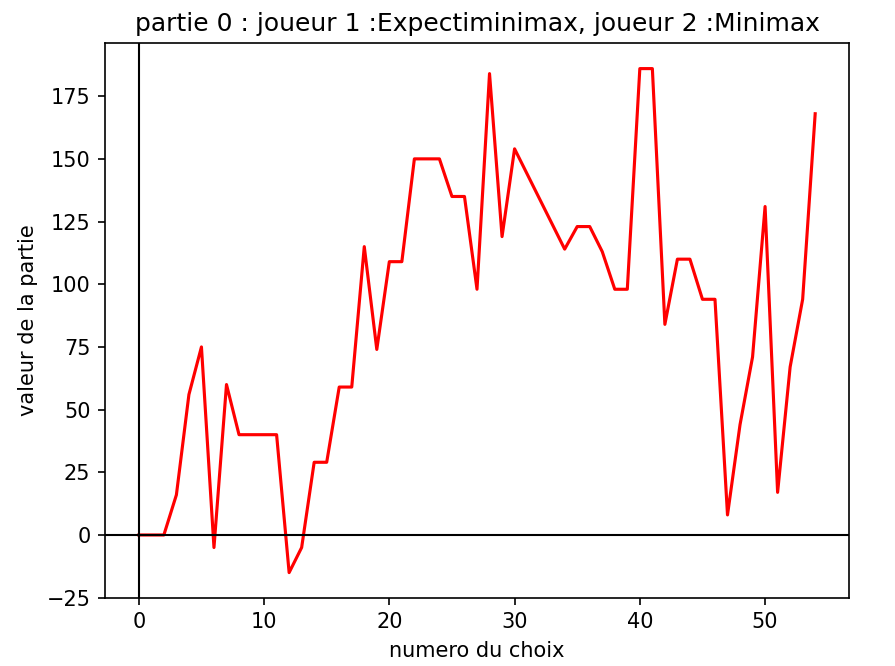
\includegraphics[width=4cm,height=4cm]{graphiques/valeur_alphbet2_alphabet2}
			    
			    Un exemple de temps de réponse: Cette fois il diminue bien en fin de partie.
                
                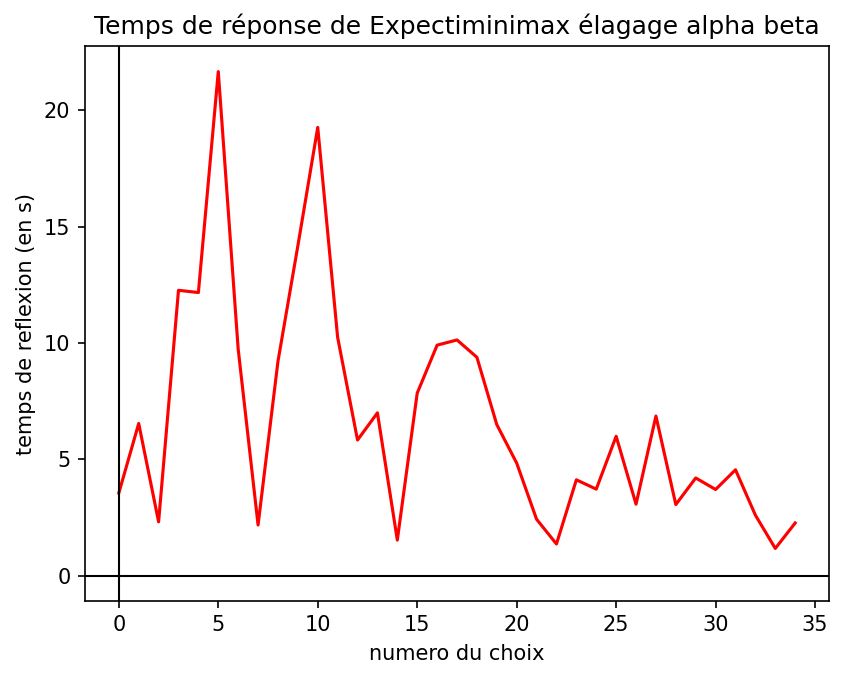
\includegraphics[width=4cm,height=4cm]{graphiques/temps_alphbet2_alphabet1}
            \paragraph{Avantages :}
                L'agent prend mieux en compte le facteur chance et fait moins d'erreurs.
                
                La solution proposée est toujours aussi générale, elle peut s'appliquer à tout les jeux à information parfaite, avec atomicité des tours.
            
            \paragraph{Desavantages :}
                Cette amélioration s'est faite au prix d'une augmetation du temps de réponse. 
                
                La faible profondeur de recherche reste une limite importante.
                
                L'agent est trés prévisible en début de partie, sachant qu'il prend toujours pikachou en premier, l'adversaire peut choisir son contre.
                
        \subsection{Ordre des mouvements}
            L'ordre de traitement des mouvements a une importance capitale pour l'élagage alpha beta. Plus un noeud correspondant à une valeur élevée est visité tôt, plus il entrainera de coupures.
            Une pratique habituelle pour trier les mouvements est de faire une recherche superficielle (c'est à dire utiliser l'algorithme du minimax avec une profondeur de 1), avant d'appliquer l'algorithme du minimax.
            \paragraph{Implementation :}
                \lstinputlisting[language=Python, tabsize=1,basicstyle=\scriptsize , linerange=tri\_mvt-end,includerangemarker=false]{code/jeu.py}
            \paragraph{Resultat :}
                Dans le cas de notre jeu, une recherche superficielle demande trop de calculs par rapport au temps gagné par les coupures suplémentaires qu'elle entraine.
                Ainsi, on observe pour tout les agents utilisant le minimax, une augmentation du temps de recherche lorsqu'on trie au préalable à la profondeur 0. 
                (Pour trier à la profondeur 0, il faut donner à la variable condition\_tri l'expression : lambda profondeur : profondeur <=1 au lieu de lambda p : False).
                Exemple : Voici le temps de reponse de l'agent expectiminimax contre l'agent minimax, avec tri à droite et sans tri à gauche.
            
            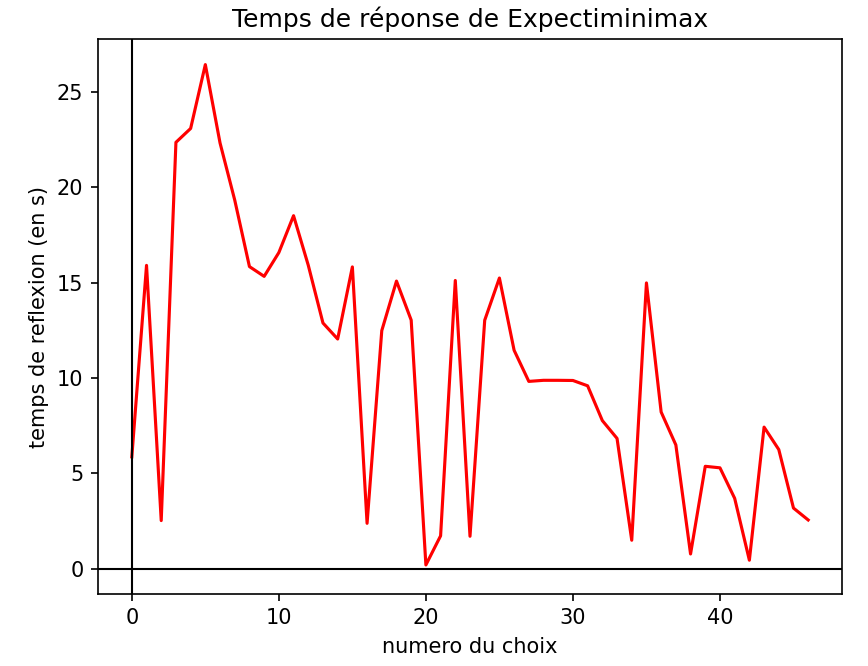
\includegraphics[width=4cm,height=4cm]{graphiques/temps_alphbet2_alphabet_tri}
            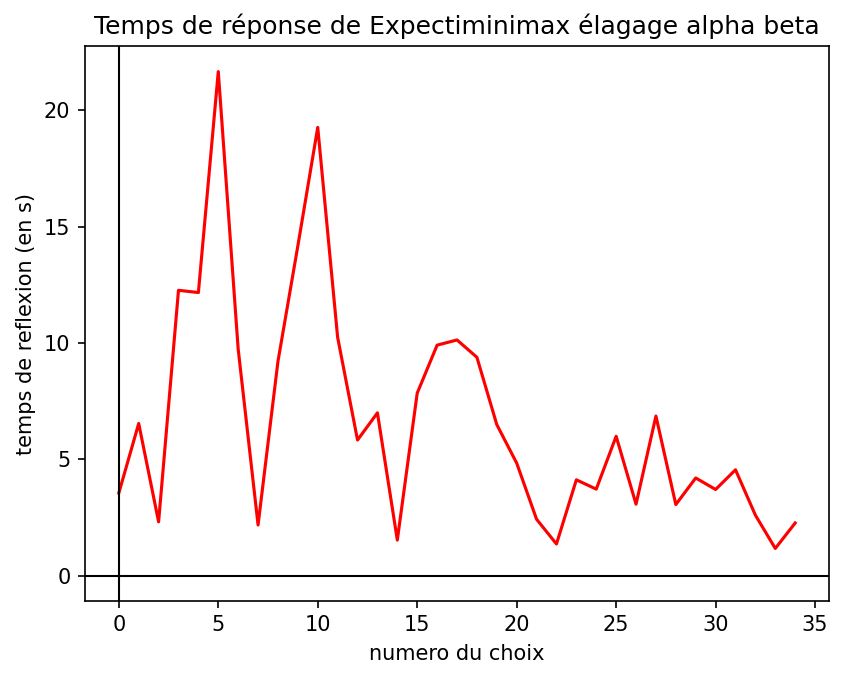
\includegraphics[width=4cm,height=4cm]{graphiques/temps_alphbet2_alphabet1}
            
            On voit que avec le tri les délais sont plus long. On trouve des résultats similaire pour l'agent minimax.
    \subsection{Solutions Envisageables}
        Deux mois de projet c'est une longue periode pour un projet scolaire, mais avec un sujet aussi vaste, il reste toujours des pistes à creuser, des détails à peaufiner. Cette section sera donc dédiée à des pistes que nous aurions voulu explorer sans pour autant avoir le temps de le faire.
        \subsubsection{Ordre des mouvements}
            Un des plus grand défaults des ia les plus performentes que nous avons réussit à coder est le temps de reponse. 
            Avec un temps de réponse plus court, on pourrait soit améliorer l'experience utilisateur, soit augmeter la profondeur de recherche et avoir une ia plus performante.
            Ainsi, pour les améliorer nos ia, un bon tri des mouvements avant les recherches serait interressant. Pour cela, on pourrait utiliser deux choses :
            \begin{itemize}
				\item Un table de hashage qui stocke les mouvements les plus efficaces qui sont a tester en premier.
				\item Lorsque deux etats ne différent que de par un facteur chance et qu'on a déjà fait l'algorithme du minimax pour le premier, on peut stocker le mouvement résultant et l'explorer en premier. Souvent deux etats qui ne différent que d'un facteur chance sont trés proches et le mouvement stocké sera le bon créant donc de nombreuses coupures.
			\end{itemize}
		\subsubsection{Recherche de principale variation}
		    Toujours dans l'idée de réduire le temps de calcul, on pourrait se pencher sur un amélioration de l'algorithme alpha beta qui est nommé recherche de principale variation ou PVS (Principal Variation Search).
		    C'est un algorithme qui repose sur un bon tri préalable des mouvements c'est pourquoi le point précédent sera important.
		    Il se déroule de la manière suivante:
		    \begin{itemize}
				\item On tri les mouvements disponibles.
				\item Pour le premier mouvement on fait une recherche complète avec l'algorithme minimax
				\item Pour tout les autres on fait une recherche de fenetre nulle (zero window search). C'est une recherche pour laquelle beta = alpha + 1. Ce type de recherche produit bien plus de coupure que l'élagage alpha beta et ne renvoie qu'une information : est-ce que le mouvement améliore la valeur actuelle.
				\item Pour tout les mouvements qui ont améliorer la valeur actuelle, on effectue une recherche complète.
				\item On remonte la valeur de la recherche complète qui est la plus grande pour le max et la plus petite pour le min.
			\end{itemize}
			Ainsi, si l'ordre des mouvements est bon on aura fait trés peu de recherches complètes et une majorite de recherches à fenetre nulle et on aura économiser un temps précieux.